\documentclass{beamer}
\usepackage[german]{babel}
\usepackage[utf8]{inputenc}

\input{Header.txt}

\usepackage[
	backend=biber,   % use modern biber backend
	autolang=hyphen, % load hyphenation rules for if language of bibentry is not
	sorting=none,    % german, has to be loaded with \setotherlanguages
	maxbibnames=4,   % in the references.bib use langid={en} for english sources
]{biblatex}
\addbibresource{Literatur.bib}
\DefineBibliographyStrings{english}{andothers = {{et\,al\adddot}}} 

\title{Flavour Mixing Effects in the Direct Detection of Dark Matter}
\author{Anja Beck}
\date{1. August 2017}
\institute{Lehrstuhl für Theoretische Physik IV \\ Fakultät Physik \\ Technische Universität Dortmund}


\begin{document}

\begin{frame}[plain,noframenumbering]
\hspace*{-0.75cm}\parbox[t]{\textwidth}{
	\titlepage}
\end{frame}

\begin{frame}[noframenumbering]{Inhalt}
	\tableofcontents{}
\end{frame}

\section{Einführung}
\begin{frame}{Dunkle Materie}
	\begin{figure}
	\centering
	\resizebox{.8\textwidth}{!}{
	\begin{tikzpicture}
		\pie[
		color={yellow, green, cyan},
		radius=2.5,
		text=legend,
%		explode={0,0,0}
		]{4.9/Gewöhnliche Materie, 26.8/ Dunkle Materie, 68.3/ Dunkle Energie}
	\end{tikzpicture}}
	\caption{Energieverteilung im Universum (ESA, Planck Teleskop 2013)}
\end{figure}
\end{frame}

\begin{frame}{Direct Detection}
	\begin{figure}[H]
		\resizebox{.6\textwidth}{!}{
			\begin{tikzpicture}
\tikzstyle{centerArrow}=[decoration={
    markings,
    mark=at position 0.5 with {\fill (2pt,0)--(-2pt,2.31pt)--(-2pt,-2.31pt)--cycle;}}]
\begin{scope}
\def\xmove{2.5}
\def\ymove{1.25}
\def\centerSize{0.15}
\node [fill, circle,inner sep=\centerSize cm] (tCenter)  {};
\node (upperLeft) at (-\xmove,\ymove) {$\chi$};
\node (upperRight) at (\xmove,\ymove) {$\chi$};
\node (lowerLeft) at (-\xmove,-\ymove) {$N$};
\node (lowerRight) at (\xmove,-\ymove) {$N$};
\draw [centerArrow,postaction={decorate}]  (upperLeft) -- (tCenter) ;
\draw [centerArrow,postaction={decorate}]  (lowerLeft) -- (tCenter) ;
\draw [centerArrow,postaction={decorate}]  (tCenter) -- (upperRight) ;
\draw [centerArrow,postaction={decorate}]  (tCenter) -- (lowerRight) ;
\end{scope}
\end{tikzpicture}
		}
		\caption{Streuung eines DM-Teilchens am Atomkern.}
	\end{figure}
\end{frame}
\section{Flavour-Mischung}
\begin{frame}{Flavour-Mischung}
\end{frame}
\section{Verwendeter Formalismus}
\begin{frame}{Formalismus}
\framesubtitle{Operatoren}
Unchirale Operatoren:
\begin{align*}
	R_{1,q} &= (\bar{\chi}\gamma_\mu\chi)(\bar{q}\gamma^\mu q) && &R_{3,q} &= (\bar{\chi}\gamma_\mu\chi)(\bar{q}\gamma^\mu\gamma_5q) \\
	R_{2,q} &= (\bar{\chi}\gamma_\mu\gamma_5\chi)(\bar{q}\gamma^\mu q) &&	&R_{4,q} &= (\bar{\chi}\gamma_\mu\gamma_5\chi)(\bar{q}\gamma^\mu\gamma_5q)
\end{align*}
Chirale Operatoren:
\begin{align*}
	Q_{1ij} &= (\bar{\chi}\gamma_\mu\tilde{\tau}^3\chi)(\bar{Q}_L^i\gamma^\mu \tau^3Q_L^j) && &Q_{5ij} &= (\bar{\chi}\gamma_\mu\gamma_5\tilde{\tau}^3\chi)(\bar{Q}_L^i\gamma^\mu \tau^3Q_L^j) \\
	Q_{2ij} &= (\bar{\chi}\gamma_\mu\chi)(\bar{Q}_L^i\gamma^\mu Q_L^j) && &Q_{6ij} &= (\bar{\chi}\gamma_\mu\gamma_5\chi)(\bar{Q}_L^i\gamma^\mu Q_L^j) \\
	Q_{3ij} &= (\bar{\chi}\gamma_\mu\chi)(\bar{U}_R^i\gamma^\mu U_R^j) && &Q_{7ij} &= (\bar{\chi}\gamma_\mu\gamma_5\chi)(\bar{U}_R^i\gamma^\mu U_R^j) \\
	Q_{4ij} &= (\bar{\chi}\gamma_\mu\chi)(\bar{D}_R^i\gamma^\mu D_R^j) && &Q_{8ij} &= (\bar{\chi}\gamma_\mu\gamma_5\chi)(\bar{D}_R^i\gamma^\mu D_R^j)
\end{align*}
\textbf{Ziel:} Drücke die Koeffizienten der unchiralen Operatoren in Abhängigkeit der Koeffizienten der chiralen Operatoren aus.
\end{frame}


\begin{frame}{Formalismus}
\framesubtitle{Rechnung: Schritt 1}
Einfügen der CKM-Matrix:
\begin{align*}
	\bar{Q}_L^i\gamma^\mu Q_L^j &= \bar{U}_L^i\gamma^\mu U_L^j + \bar{D}_L^i\gamma^\mu D_L^j \\
	&= \bar{U}_L^i\gamma^\mu U_L^j \\
	&+ (V_{id}^*\bar{d}_L + V_{is}^*\bar{s}_L+V_{ib}^*\bar{b}_L)\gamma^\mu(V_{jd}d_L+V_{js}s_L+V_{jb}b_L) \\
	&= \bar{u}_L\gamma^\mu u_L\delta_{ij}\delta_{iu} + V_{id}^*V_{jd}\bar{d}_L\gamma^\mu d_L + V_{is}^*V_{js}\bar{s}_L\gamma^\mu s_L
\end{align*}
\end{frame}


\begin{frame}{Formalismus}
\framesubtitle{Rechnung: Schritt 2}
Umschreiben der chiralen Teilchen-Multipletts mit den links- und rechtshändigen Projektoren:
\begin{align*}
	\bar{Q}_L^i\gamma^\mu Q_L^j &=\frac{1}{2}(
	\bar{u}\gamma^\mu u\delta_{iu}\delta_{ij} + V_{id}^*V_{jd}\bar{d}\gamma^\mu d
	+ V_{is}^*V_{js}\bar{s}\gamma^\mu s) \\
	&- \frac{1}{2}(\bar{u}\gamma^\mu\gamma_5u\delta_{iu}\delta_{ij} + V_{id}^*V_{jd}\bar{d}\gamma^\mu\gamma_5d + V_{is}^*V_{js}\bar{s}\gamma^\mu\gamma_5s)
\end{align*}
Identifikation der nicht-chiralen Operatoren:
\begin{align*}
	Q_{2ij} &= \frac{1}{2}(R_{1u}\delta_{iu}\delta_{ij}+ V_{id}^*V_{jd}R_{1d}+ V_{is}^*V_{js}R_{1s}) \notag \\
	&- \frac{1}{2}(R_{3u}\delta_{iu}\delta_{ij} + V_{id}^*V_{jd}R_{3d} + V_{is}^*V_{js}R_{3s})
\end{align*}
\end{frame}


\begin{frame}{Formalismus}
\framesubtitle{Rechnung: Schritt 3}
Aufstellen des Lagrangian:
\begin{align*}
	\sum_{l,q} K_{l,q}R_{l,q} \overset{!}{=} \sum_{m,i,j}C_{mij}Q_{mij}
\end{align*}
Nach dem Umsortieren der rechten Seite nach $R_{l,q}$ liefert ein Koeffizienten-Vergleich die Abhängigkeiten $K_{l,q}(C_{mij})$.
\note{Warum ist die Abhängigkeit interessant?}
\end{frame}
\section{Neue Wechselwirkung}
\begin{frame}{Neue Wechselwirkung}
\begin{itemize}
	\setlength\itemsep{1em}
	\item Neue $U(1)$-Symmetrie mit Eichboson $Z'$ \cite{InColour}
	\item Unter der neuen Wechselwirkung geladene Teilchen:
	\begin{itemize}
		\item Leptonen der zweiten und dritten Generation
		\item Neue Quarks
		\item Dunkle Materie \cite{Z}
	\end{itemize}
	\item Ein paar Worte zu $L_\mu-L_\tau$.
\end{itemize}
\end{frame}

\begin{frame}{Neue Wechselwirkung}
\framesubtitle{Kopplung der neuen Quarks an die SM-Quarks}
\begin{figure}
	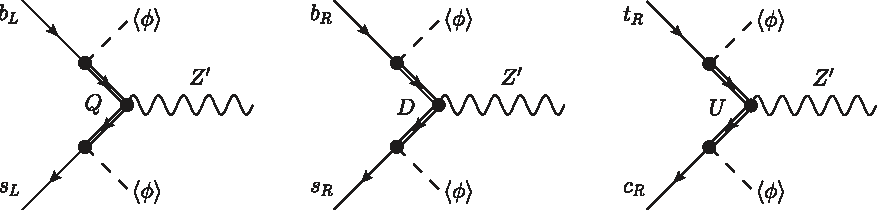
\includegraphics[width=\textwidth]{Bilder/NeueQuarks.pdf}
	\caption{Wechselwirkung von SM-Quarks mit dem Eichboson $Z'$ (aus \cite{InColour})}
\end{figure}
\end{frame}


\begin{frame}{Neue Wechselwirkung}
\framesubtitle{Erklärung seltener $B$-Zerfälle}
\begin{minipage}{.5\textwidth}
\begin{figure}
	\centering
	\resizebox{\textwidth}{!}{
	\begin{tikzpicture}
\tikzstyle{centerArrow}=[decoration={
	markings,
	mark=at position 0.5 with {\fill (2pt,0)--(-2pt,2.31pt)--(-2pt,-2.31pt)--cycle;}}]
\begin{scope}%[yshift=5cm]
\def\xmove{2.5}
\def\ymove{1.25}
\def\centerSize{0.18}

\node [fill, circle,inner sep=\centerSize cm] (tCenter) {};
\node (Left) at (-\xmove,0) {$b$};
\node (upperRight) at (\xmove,0.5*\ymove) {$s$};
\node (middleRight) at (\xmove,0) {$\mu$};
\node (lowerRight) at (\xmove,-0.5*\ymove) {$\bar{\mu}$};

\draw [centerArrow,postaction={decorate}]  (Left) -- (tCenter) ;
\draw [centerArrow,postaction={decorate}]  (tCenter) -- (upperRight) ;
\draw [centerArrow,postaction={decorate}]  (tCenter) -- (middleRight) ;
\draw [centerArrow,postaction={decorate}]  (lowerRight) -- (tCenter) ;

\node (indep1) at (-\xmove, \ymove) {$\bar{u},\bar{d},\bar{s}$};
\node (indep2) at (\xmove, \ymove) {$\bar{u},\bar{d},\bar{s}$};
\draw [centerArrow,postaction={decorate}] (indep2) -- (indep1);

\end{scope}
\end{tikzpicture}
	}
	\caption{$B\rightarrow K\mu\bar{\mu}$ bzw. $B_s\rightarrow \Phi\mu\bar{\mu}$}
\end{figure}
\end{minipage}
\hfill
\begin{minipage}{.45\textwidth}
\begin{figure}
	\centering
	\resizebox{\textwidth}{!}{
		\begin{tikzpicture}
\tikzstyle{centerArrow}=[decoration={
	markings,
	mark=at position 0.5 with {\fill (2pt,0)--(-2pt,2.31pt)--(-2pt,-2.31pt)--cycle;}}]
\begin{scope}%[xshift=-8cm]
\def\xmove{2.5}
\def\ymove{0.5}
\def\centerSize{0.08}

\node [fill, circle, inner sep=\centerSize cm] (tCenter1)  {};
\coordinate (tCenter2) at (1,-1cm);
\node (Left) at (-\xmove,0) {$b$};
\node (upperRight) at (\xmove,0) {$s$};
\node (middleRight) at ([xshift=1.5cm,yshift=\ymove cm] tCenter2) {$\mu$};
\node (lowerRight) at ([xshift=1.5cm,yshift=-\ymove cm] tCenter2) {$\bar{\mu}$};


\draw [centerArrow,postaction={decorate}]  (Left) -- (tCenter1) ;
\draw [centerArrow,postaction={decorate}]  (tCenter1) -- (upperRight) ;
\draw [centerArrow,postaction={decorate}]  (tCenter2) -- (middleRight) ;
\draw [centerArrow,postaction={decorate}]  (lowerRight) -- (tCenter2) ;
\draw [decoration={snake, segment length=1.5mm, amplitude=0.5mm},decorate] (tCenter1) -- (tCenter2) ;
\end{scope}
\end{tikzpicture}
	}
	\caption{$b\rightarrow s\mu\bar{\mu}$}
\end{figure}
\end{minipage}
Beschreibung mit $Z'$-Austausch:
	\[ H = \frac{Y_{Qb}Y_{Qs}^*}{2m_Q^2}(\bar{s}_L\gamma_\mu b_L)(\bar{\mu}\gamma^\mu\mu)-\frac{Y_{Db}Y_{Ds}^*}{2m_D^2}(\bar{s}_R\gamma_\mu b_R)(\bar{\mu}\gamma^\mu\mu) \]
Beschränkung der Masse auf:
\[ m_{Q,D} \approx \SI{25}{\tera\electronvolt}\sqrt{\text{Re}\left(Y_{(Q,D)b}Y_{(Q,D)s}\right)} \]
\end{frame}


\begin{frame}{Neue Wechselwirkung}
\framesubtitle{Loop-Diagramm zur Streuung am Atomkern}
\begin{minipage}{.25\textwidth}
%	\begin{figure}[H]
		\resizebox{1.4\textwidth}{!}{
			\begin{tikzpicture}
\tikzstyle{centerArrow}=[decoration={
	markings,
	mark=at position 0.5 with {\fill (2pt,0)--(-2pt,2.31pt)--(-2pt,-2.31pt)--cycle;}}]

\begin{scope}[xshift=6cm,yshift=5cm]
\def\xmove{2}
\def\ymove{1.25}
\def\centerShift{2cm}
\def\centerCircle{1cm}
\def\centerSize{0.05cm}
\coordinate (tCenter1) at (0,0);
\coordinate (tCenter2) at (0,-\centerShift);
\coordinate (tCenter3) at (0,-\centerShift-\centerCircle);
\coordinate (tCenter4) at (0,-\centerShift-\centerCircle-\centerShift);

\node (upperLeft) at (-\xmove,\ymove) {$\chi$};
\node (upperRight) at (\xmove,\ymove) {$\chi$};
\node (lowerLeft) at (-\xmove,-\centerShift-\centerCircle-\centerShift-\ymove cm) {$N$};
\node (lowerRight) at (\xmove,-\centerShift-\centerCircle-\centerShift-\ymove cm) {$N$};

\draw [centerArrow,postaction={decorate}]  (upperLeft) -- (tCenter1) ;
\draw [centerArrow,postaction={decorate}]  (tCenter1) -- (upperRight) ;
\draw [centerArrow,postaction={decorate}]  (lowerLeft) -- (tCenter4) ;
\draw [centerArrow,postaction={decorate}]  (tCenter4) -- (lowerRight) ;
\draw [decoration={snake, segment length=1.5mm, amplitude=0.5mm},decorate] (tCenter1) -- (tCenter2) ;
\node at (0.5,-\centerShift/2) {$Z'$};
\draw [
        decoration={markings, mark=at position 0.5 with {\fill (2pt,0)--(-2pt,2.31pt)--(-2pt,-2.31pt)--cycle;}, mark=at position 1 with {\fill (2pt,0)--(-2pt,2.31pt)--(-2pt,-2.31pt)--cycle;}},
        postaction={decorate}
] ([yshift=.5cm]tCenter3) ellipse(.45 and 0.5);
\node at ([yshift=-\centerCircle/2,xshift=0.75cm]tCenter2) {$l$};
\node at ([yshift=-\centerCircle/2,xshift=-0.75cm]tCenter2) {$l$};
\draw [decoration={snake, segment length=1.5mm, amplitude=0.5mm},decorate] (tCenter3) -- (tCenter4) ;
\node at (0.5,-\centerShift/2-\centerCircle-\centerShift) {$\gamma$};
\end{scope}
\end{tikzpicture}
		}
		%		\captionsetup{width=\textwidth}
%		\caption{Loop-Wechselwirkung zur Streuung DM am Atomkern.}
%	\end{figure}
\end{minipage}
\hfill
\begin{minipage}{.7\textwidth}
	Wirkungsquerschnitt ohne Impulsübertrag:
	\[ \sigma_\text{0,loop} = \frac{\mu_{A\chi}^2}{A^2\pi}\left(\frac{\alpha_{em}Z}{3\pi}\ \frac{g'^2q_\chi q_l}{m_{Z'}^2}\log\left(\frac{m_\mu^2}{m_\tau^2}\right)\right)^2 \]
\end{minipage}
\end{frame}


\begin{frame}{Neue Wechselwirkung}
\framesubtitle{Beschränkung der Parameter}
Weitere $B$-Zerfälle:
\[ \SI{540}{\giga\electronvolt}\lessapprox\frac{m_{Z'}}{g'}\lessapprox\SI{4.9}{\tera\electronvolt} \]
Relic Density:
	\[ m_{Z'}\approx 2m_\chi \]
Direct Detection $(q_\chi=q_l)$:
	\[ \SI{10}{\giga\electronvolt}\lessapprox m_{Z'} \lessapprox\SI{46}{\giga\electronvolt} \]
	\[ \SI{2e-3}{}\lessapprox g' \lessapprox\SI{e-2}{} \]
\end{frame}
\section{Ergebnisse}
\begin{frame}{Direct Detection mit Flavour-Mischung}
	Annahmen: DM koppelt ausschließlich an $Z'$. Von den Quarks wechselwirken nur $s,b$ mit $Z'$. \\
	\resizebox{.5\textwidth}{!}{
		\begin{tikzpicture}
\tikzstyle{centerArrow}=[decoration={
markings,
mark=at position 0.5 with {\fill (2pt,0)--(-2pt,2.31pt)--(-2pt,-2.31pt)--cycle;}}]
\begin{scope}[xshift=3cm,yshift=-2cm]
\def\xmove{2}
\def\ymove{1.25}
\def\centerShift{2}
\def\centerSize{0.08cm}
\coordinate (tCenter1) at (0,0);
\coordinate[fill, circle,inner sep=\centerSize] (tCenter2) at (0,-\centerShift cm);
\node (upperLeft) at (-\xmove,\ymove) {$\chi$};
\node (upperRight) at (\xmove,\ymove) {$\chi$};
\node (lowerLeft) at (-\xmove,-\centerShift cm-\ymove cm) {$b_L,s_L$};
\node (lowerRight) at (\xmove,-\centerShift cm-\ymove cm) {$s_L,b_L$};
\node at (0.5,-\centerShift/2) {$Z'$};
\draw [centerArrow,postaction={decorate}]  (upperLeft) -- (tCenter1) ;
\draw [centerArrow,postaction={decorate}]  (tCenter1) -- (upperRight) ;
\draw [centerArrow,postaction={decorate}]  (lowerLeft) -- (tCenter2) ;
\draw [centerArrow,postaction={decorate}]  (tCenter2) -- (lowerRight) ;
\draw [decoration={snake, segment length=1.5mm, amplitude=0.5mm},decorate] (tCenter1) -- (tCenter2) ;
\end{scope}
\end{tikzpicture}
	}
\end{frame}


\begin{frame}{Schranken aus dem $B$-Zerfall 1}
\framesubtitle{Real- und Imaginärteil variabel}
	\begin{figure}
		\centering
		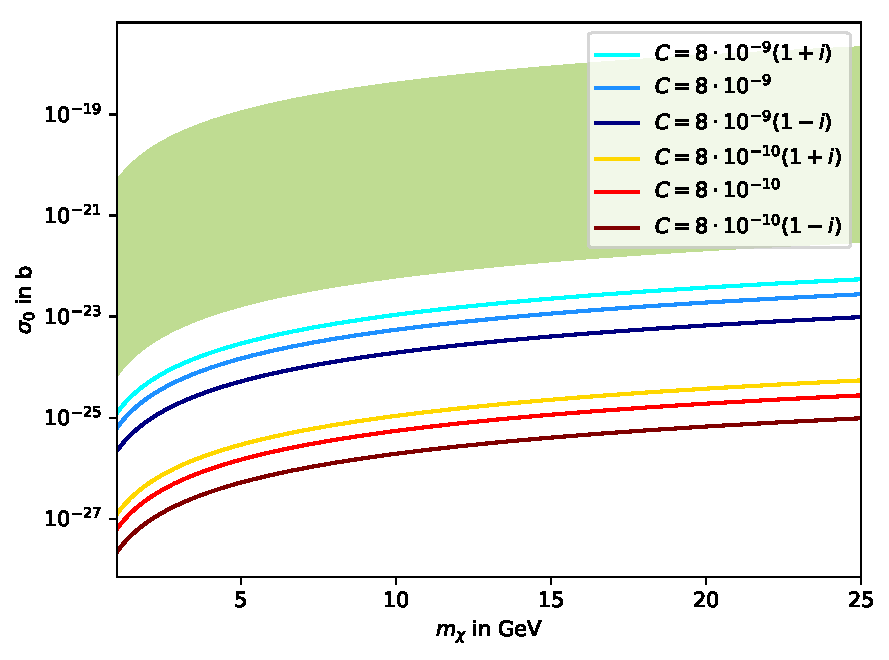
\includegraphics[width=.8\textwidth]{Bilder/Allgemein11.pdf}
		\caption{$q_l=q_\chi=1$}
	\end{figure}
\end{frame}
\begin{frame}[noframenumbering]{Schranken aus dem $B$-Zerfall 1}
\framesubtitle{Real- und Imaginärteil variabel}
	\begin{figure}
		\centering
		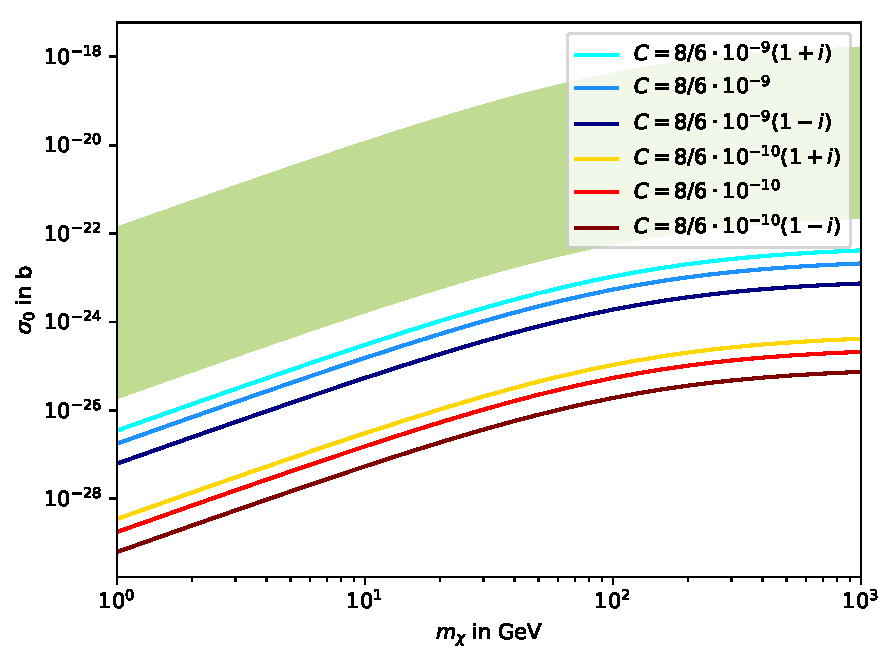
\includegraphics[width=.8\textwidth]{Bilder/Allgemein116.pdf}
		\caption{$q_l=1,q_\chi=\sfrac{1}{6}$}
	\end{figure}
\end{frame}


\begin{frame}{Schranken aus dem $B$-Zerfall 2}
\framesubtitle{Fester Realteil, variabler Imaginärteil}
	\begin{figure}
		\centering
		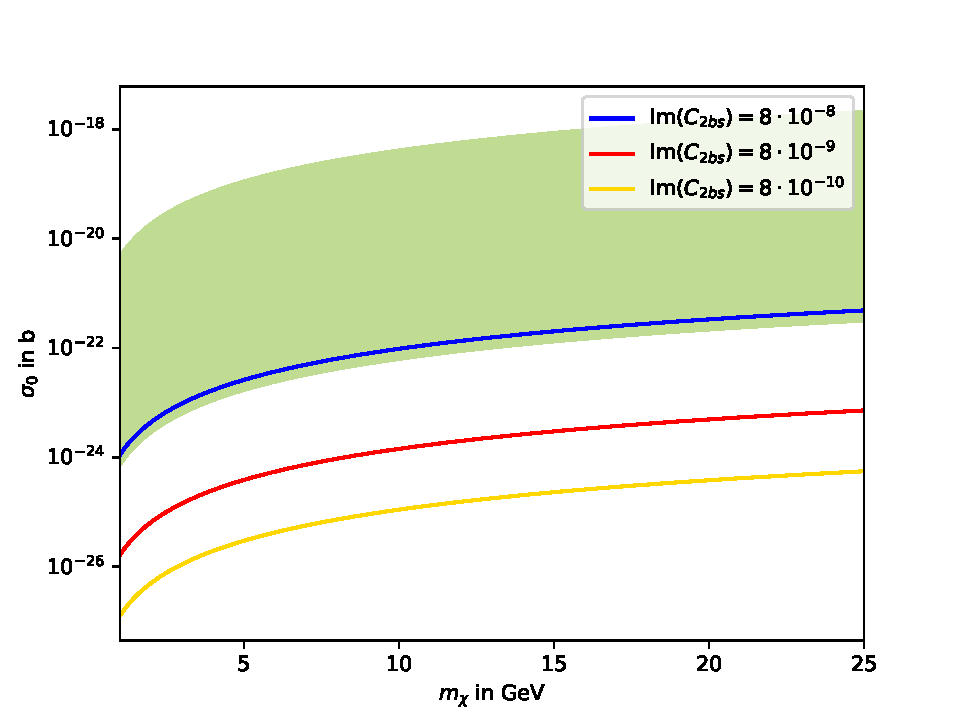
\includegraphics[width=.8\textwidth]{Bilder/Im11.pdf}
		\caption{$q_l=q_\chi=1$}
	\end{figure}
\end{frame}
\begin{frame}[noframenumbering]{Schranken aus dem $B$-Zerfall 2}
\framesubtitle{Fester Realteil, variabler Imaginärteil}
	\begin{figure}
		\centering
		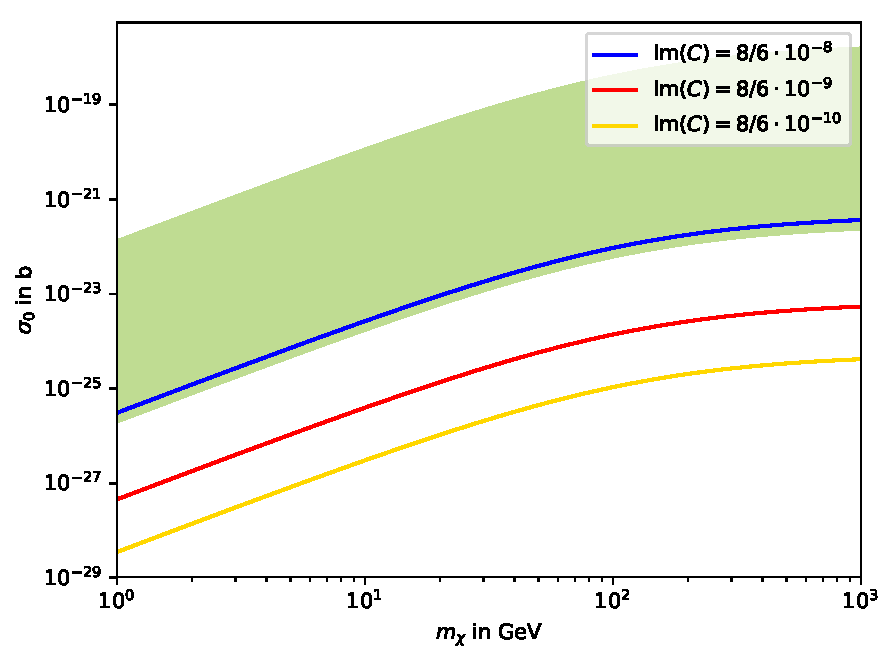
\includegraphics[width=.8\textwidth]{Bilder/Im116.pdf}
		\caption{$q_l=1,q_\chi=\sfrac{1}{6}$}
	\end{figure}
\end{frame}


\begin{frame}{Schranken aus der Relic Density}
\begin{figure}
	\centering
	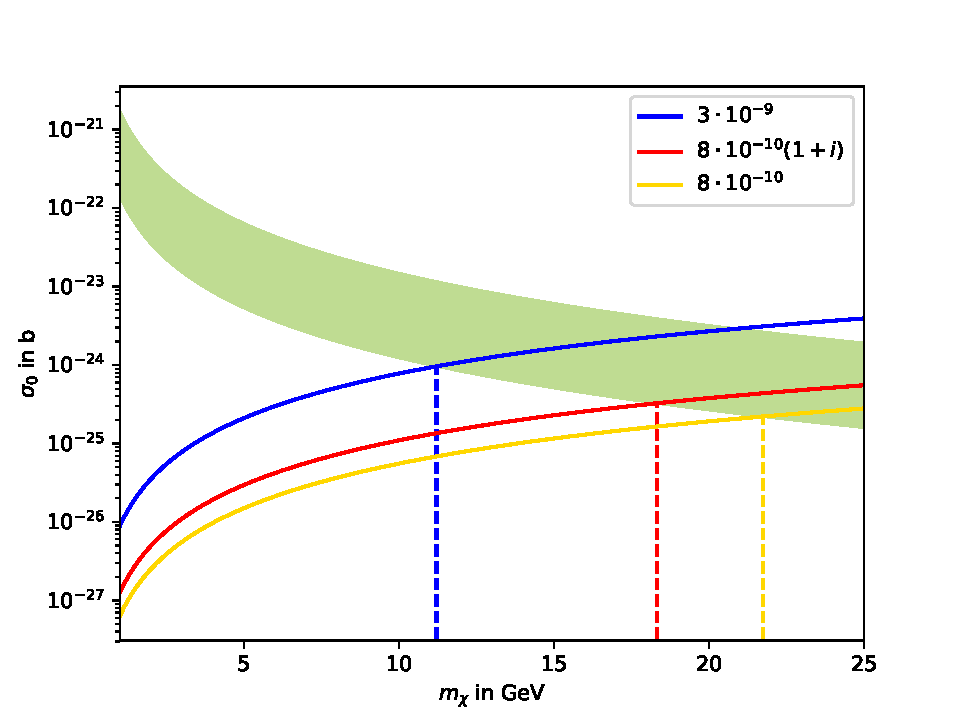
\includegraphics[width=.8\textwidth]{Bilder/Relic11.pdf}
	\caption{$q_l=q_\chi=1$}
\end{figure}
\end{frame}
\begin{frame}[noframenumbering]{Schranken aus der Relic Density}
\begin{figure}
\centering
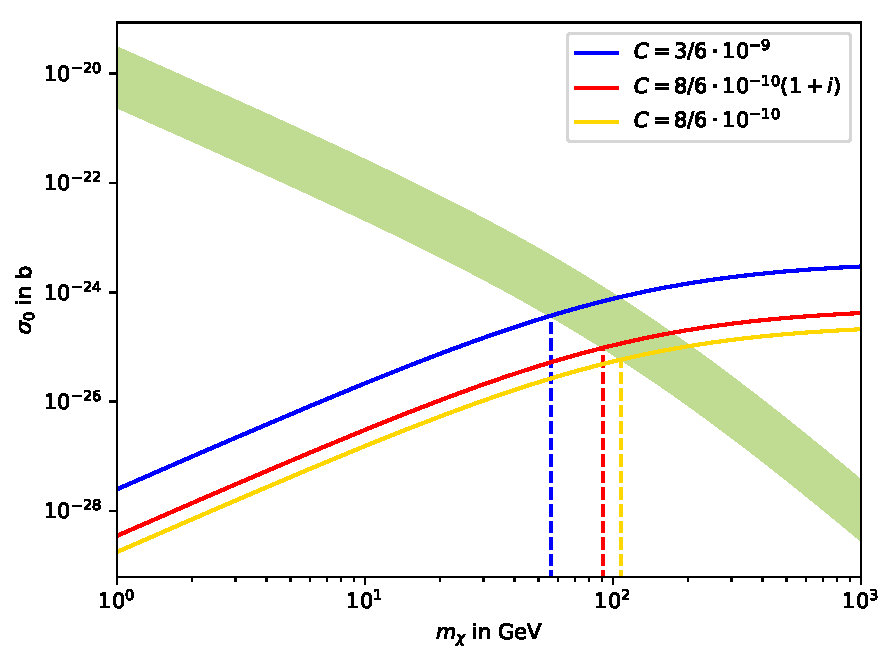
\includegraphics[width=.8\textwidth]{Bilder/Relic116.pdf}
\caption{$q_l=1,q_\chi=\sfrac{1}{6}$}
\end{figure}
\end{frame}

\section{Bibliographie}
\begin{frame}{Bibliographie}
	\printbibliography
\end{frame}
\end{document}


